\section{Additional Treatment Effects Tables \& Effect Plots} \label{sec:appxa}

\subsection{Full set of Treatment Effects for Housing Prices}

The full set of treatment effects provided in Table \ref{tab:median_sale_amount_full} support Table \ref{tab:median_sale_amount} which provides treatment effects for the housing price outcome variable in the main body of the paper. These treatment effects are estimated using a regression model that controls for various factors.

\begin{table}[htbp]
    \centering
    \caption{Full set of estimates - Median Housing Price}
    \label{tab:median_sale_amount_full}
    \begin{tabular}{p{3cm}cccc}
        \hline
        \textbf{Year relative to vote} & \textbf{Estimate} & \textbf{Standard error} & \textbf{p-value} & \textbf{Confidence interval} \\
        \hline
        $t - 3$  & 3,468   & 7,465  & 0.642  & [-11,164, 18,099] \\
        $t - 2$  & -1,703  & 6,617  & 0.797  & [-14,673, 11,267] \\
        $t - 1$  & 1,784   & 6,950  & 0.797  & [-11,838, 15,407] \\
        $t + 1$ & -6,197  & 9,662  & 0.521  & [-25,134, 12,741] \\
        $t + 2$ & -17,059 & 9,518  & 0.073  & [-35,715, 1,597] \\
        $t + 3$ & -9,823  & 8,244  & 0.233  & [-25,981, 6,335] \\
        $t + 4$ & -19,535 & 9,289  & 0.035  & [-37,741, -1,329] \\
        $t + 5$ & -21,531 & 9,147  & 0.019  & [-39,459, -3,604] \\
        $t + 6$ & -16,994 & 7,558  & 0.025  & [-31,809, -2,180] \\
        $t + 7$ & -16,991 & 7,357  & 0.023  & [-31,111, -2,272] \\
        $t + 8$ & -23,323 & 9,449  & 0.014  & [-41,842, -4,803] \\
        $t + 9$ & -30,620 & 9,586  & 0.001  & [-49,408, -11,833] \\
        $t + 10$ & -16,411 & 9,342  & 0.079  & [-34,721, 1,898] \\
        \hline
    \end{tabular}
    \begin{tablenotes}
        \small
        \item Supplements Table \ref{tab:median_sale_amount} in text. Full set of treatment effect estimates of renewing road tax levies relative to cutting road tax levies from 3 years before the vote to 10 years after the vote. Covariates from Table \ref{tab:variable_means_sd} used in all regressions. Outcome is median house price in constant 2010 U.S. dollars. Unit of observation is the city-year. A treatment effect of -\$19,535 means that four years after the vote, cities that vote to cut road taxes and its associated spending have houses that sell for \$19,535 less than cities that vote to renew road taxes and spending.
    \end{tablenotes}
\end{table}

\begin{figure}[htbp]
    \centering
    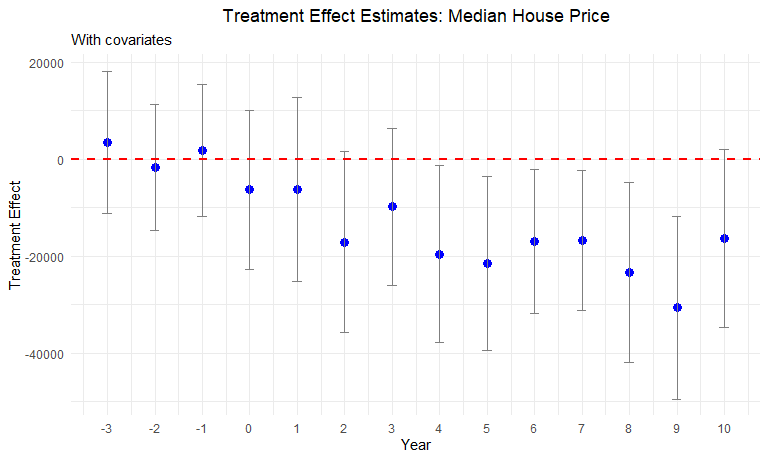
\includegraphics[width=\textwidth,keepaspectratio]{images/tes_gs.png}
    \caption{Event Study - Median Housing Price}
    \label{fig:tes_gs_app}
\end{figure}

\clearpage

\subsection{Full set of Treatment Effects for employment outcome variable}

The full set of treatment effects for the employment outcome variable for the full sample of cities have been provided below.

\begin{table}[htbp]
    \centering
    \caption{Full set of estimates - Average Employment}
    \label{tab:average_employment}
    \begin{tabular}{lcccc}
        \hline
        Year relative to vote & Estimate & Standard error & p-value & Confidence interval \\
        \hline
        $t - 3$  & 489   & 444  & 0.270  & [-380, 1359] \\
        $t - 2$  & 449   & 391  & 0.251  & [-317, 1215] \\
        $t - 1$  & 429   & 373  & 0.249  & [-301, 1160] \\
        $t + 1$ & 400   & 347  & 0.250  & [-281, 1080] \\
        $t + 2$ & 173   & 295  & 0.558  & [-406, 752] \\
        $t + 3$ & 68    & 313  & 0.827  & [-545, 682] \\
        $t + 4$ & -24   & 319  & 0.939  & [-650, 601] \\
        $t + 5$ & -100  & 343  & 0.771  & [-772, 572] \\
        $t + 6$ & -357  & 324  & 0.271  & [-993, 278] \\
        $t + 7$ & -384  & 304  & 0.206  & [-980, 211] \\
        $t + 8$ & -281  & 311  & 0.366  & [-891, 329] \\
        $t + 9$ & -237  & 350  & 0.497  & [-922, 448] \\
        $t + 10$ & -406  & 372  & 0.275  & [-1135, 323] \\
        \hline
    \end{tabular}
    \begin{tablenotes}
        \small
        \item Full set of estimates of the treatment effect on average employment for areas renewing versus cutting road tax levies, from 3 years before to 10 years after the vote.
    \end{tablenotes}
\end{table}



\begin{figure}[htbp]
    \centering
    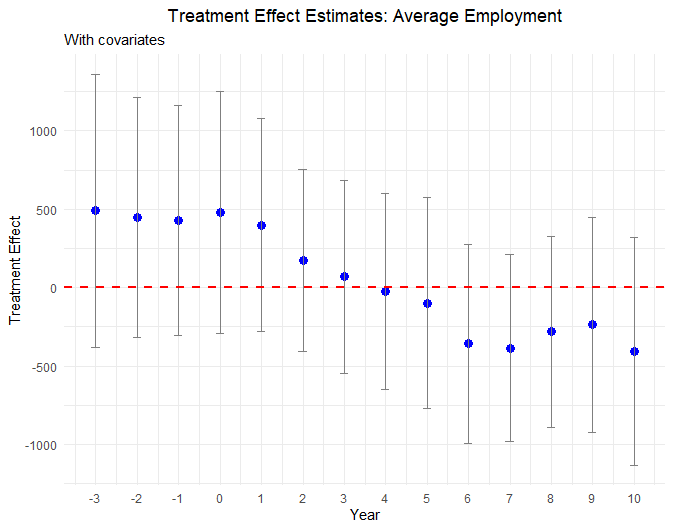
\includegraphics[width=\textwidth,keepaspectratio]{images/tes_emp.png}
    \caption{Effect plot: Average Employment}
    \label{fig:tes_gs_emp}
\end{figure}

\begin{table}[htbp]
    \centering
    \caption{Full set of estimates - Log Average Employment}
    \label{tab:log_average_employment}
    \begin{tabular}{p{3cm}cccc}
        \hline
        Year relative to vote & estimate & Standard error & p-value & Confidence interval \\
        \hline
        $t - 3$  & 0.640  & 0.438  & 0.144  & [-0.218, 1.497] \\
        $t - 2$  & 0.688  & 0.392  & 0.079  & [-0.079, 1.456] \\
        $t - 1$  & 0.641  & 0.385  & 0.096  & [-0.114, 1.397] \\
        $t + 1$ & 0.308  & 0.342  & 0.368  & [-0.363, 0.98] \\
        $t + 2$ & 0.336  & 0.304  & 0.270  & [-0.261, 0.933] \\
        $t + 3$ & 0.297  & 0.285  & 0.297  & [-0.261, 0.855] \\
        $t + 4$ & 0.201  & 0.283  & 0.478  & [-0.354, 0.756] \\
        $t + 5$ & 0.235  & 0.270  & 0.385  & [-0.295, 0.765] \\
        $t + 6$ & 0.040  & 0.236  & 0.865  & [-0.422, 0.503] \\
        $t + 7$ & 0.004  & 0.238  & 0.987  & [-0.462, 0.47] \\
        $t + 8$ & -0.077 & 0.233  & 0.741  & [-0.535, 0.38] \\
        $t + 9$ & -0.094 & 0.240  & 0.696  & [-0.564, 0.377] \\
        $t + 10$ & -0.008 & 0.281  & 0.977  & [-0.56, 0.543] \\
        \hline
    \end{tabular}
    \begin{tablenotes}
        \small
        \item Full set of estimates of the treatment effect on log average employment for areas renewing versus cutting road tax levies, from 3 years before to 10 years after the vote.
    \end{tablenotes}
\end{table}

\begin{figure}[htbp]
    \centering
    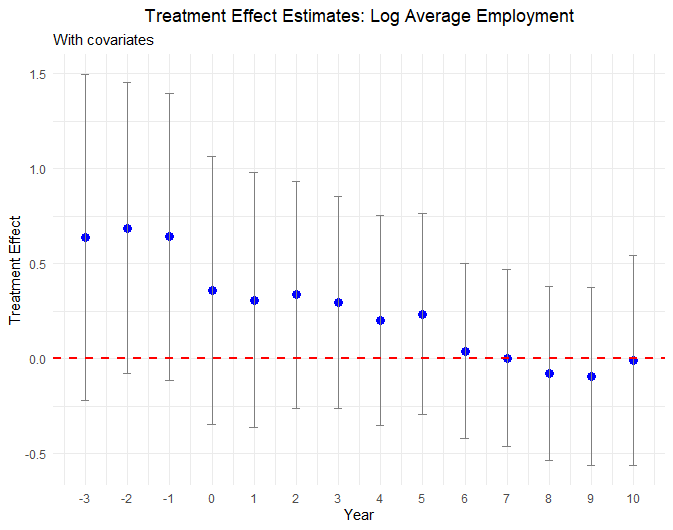
\includegraphics[width=\textwidth,keepaspectratio]{images/tes_ln_emp.png}
    \caption{Effect plot: Log Average Employment}
    \label{fig:tes_ln_emp}
\end{figure}

\clearpage

\subsection{Full set of Treatment Effects for wage outcome variable}

\begin{table}[htbp]
    \centering
    \caption{Full set of estimates - Total Wages}
    \label{tab:total_wages}
    \begin{tabular}{p{2cm}cccc}
        \hline
        Year relative to vote & Estimate & Standard error & p-value & Confidence interval \\
        \hline
        $t - 3$  & 24,989,152   & 20,849,660   & 0.231  & [-15,876,182, 65,854,486] \\
        $t - 2$  & 21,441,310   & 19,889,330   & 0.281  & [-17,541,777, 60,424,398] \\
        $t - 1$  & 19,881,825   & 19,361,782   & 0.304  & [-18,067,267, 57,830,917] \\
        $t + 1$ & 19,192,209   & 18,280,413   & 0.294  & [-16,637,400, 55,021,819] \\
        $t + 2$ & 13,929,445   & 14,858,316   & 0.349  & [-15,192,855, 43,051,744] \\
        $t + 3$ & 8,703,249    & 15,217,865   & 0.567  & [-21,123,766, 38,530,263] \\
        $t + 4$ & 4,588,179    & 15,209,473   & 0.763  & [-25,222,389, 34,398,747] \\
        $t + 5$ & 1,451,493    & 15,943,802   & 0.927  & [-29,798,358, 32,701,345] \\
        $t + 6$ & -9,929,705   & 11,649,814   & 0.394  & [-32,763,341, 12,903,931] \\
        $t + 7$ & -11,342,970  & 10,518,262   & 0.281  & [-31,958,764, 9,272,824] \\
        $t + 8$ & -8,616,720   & 10,709,258   & 0.421  & [-29,606,866, 12,373,426] \\
        $t + 9$ & -6,319,035   & 12,894,791   & 0.624  & [-31,592,825, 18,954,755] \\
        $t + 10$ & -10,837,202 & 13,975,637   & 0.438  & [-38,229,451, 16,555,046] \\
        \hline
    \end{tabular}
    \begin{tablenotes}
        \small
        \item Full set of estimates of the treatment effect on total wages for areas renewing versus cutting road tax levies, from 3 years before to 10 years after the vote.
    \end{tablenotes}
\end{table}

\begin{figure}[htbp]
    \centering
    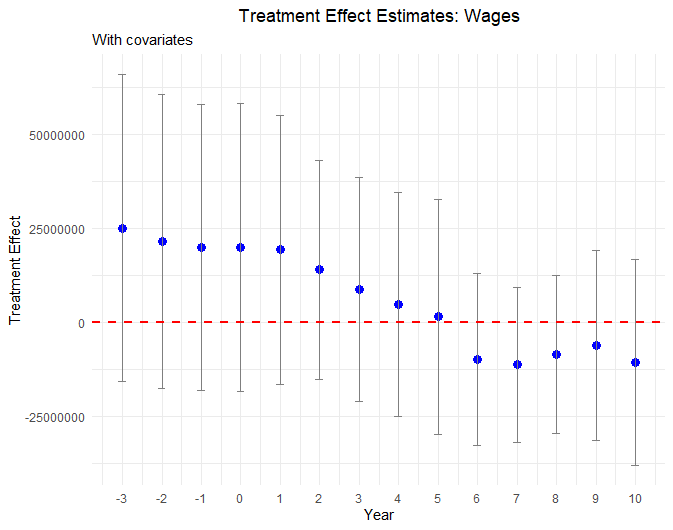
\includegraphics[width=\textwidth,keepaspectratio]{images/tes_wages.png}
    \caption{Effect plot: Wages}
    \label{fig:tes_wages}
\end{figure}


\begin{table}[htbp]
    \centering
    \caption{Full set of estimates - Log Total Wages}
    \label{tab:log_total_wages}
    \begin{tabular}{p{3cm}cccc}
        \hline
        Year relative to vote & Estimate & Standard error & p-value & Confidence interval \\
        \hline
        $t - 3$  & 0.636  & 0.496  & 0.200  & [-0.336, 1.609] \\
        $t - 2$  & 0.747  & 0.438  & 0.088  & [-0.111, 1.606] \\
        $t - 1$  & 0.740  & 0.442  & 0.094  & [-0.126, 1.605] \\
        $t + 1$ & 0.364  & 0.393  & 0.354  & [-0.406, 1.134] \\
        $t + 2$ & 0.369  & 0.348  & 0.289  & [-0.313, 1.051] \\
        $t + 3$ & 0.389  & 0.328  & 0.235  & [-0.253, 1.032] \\
        $t + 4$ & 0.230  & 0.330  & 0.485  & [-0.417, 0.877] \\
        $t + 5$ & 0.295  & 0.306  & 0.334  & [-0.304, 0.894] \\
        $t + 6$ & 0.049  & 0.262  & 0.851  & [-0.465, 0.564] \\
        $t + 7$ & 0.049  & 0.269  & 0.855  & [-0.478, 0.576] \\
        $t + 8$ & -0.031 & 0.258  & 0.905  & [-0.537, 0.475] \\
        $t + 9$ & -0.063 & 0.264  & 0.811  & [-0.58, 0.454] \\
        $t + 10$ & 0.026  & 0.306  & 0.932  & [-0.573, 0.625] \\
        \hline
    \end{tabular}
    \begin{tablenotes}
        \small
        \item Full set of estimates of the treatment effect on log total wages for areas renewing versus cutting road tax levies, from 3 years before to 10 years after the vote.
    \end{tablenotes}
\end{table}

\begin{figure}[htbp]
    \centering
    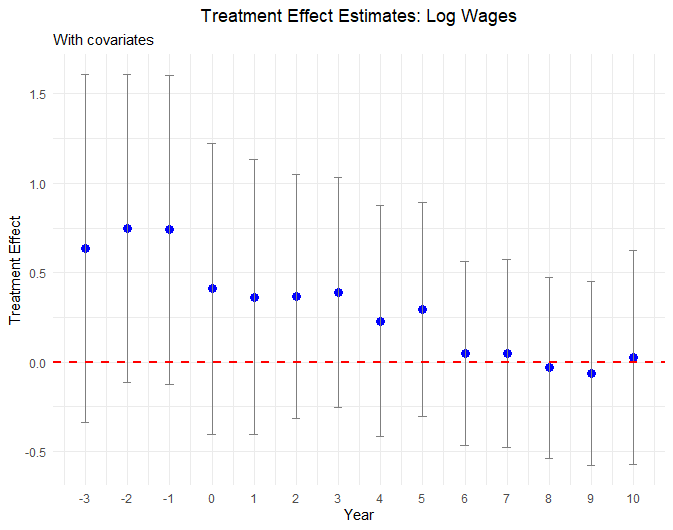
\includegraphics[width=\textwidth,keepaspectratio]{images/tes_ln_wages.png}
    \caption{Effect plot: Log Wages}
    \label{fig:tes_ln_wages}
\end{figure}

% \subsection{Outcome vs Running variable plots for years after Treatment}

\clearpage

\section{Additional Robustness Tests} \label{sec:appxb}

\subsection{Covariate Discontinuity Tests \& Smoothness Plots}

\begin{table}[!h]
    \centering
    \caption{Covariate Discontinuity Test Results}
    \label{tab:covariate_discontinuity}
    \begin{tabular}{p{2cm}cccc}
        \hline
        Variable & Estimate & Standard error & p-value & Confidence interval \\
        \hline
        Population                           & -388      & 1,094   & 0.722  & [-2,532, 1,755] \\
        Poverty Rate                         & 0.017     & 0.014   & 0.234  & [-0.011, 0.045] \\
        \% with Kids                         & -0.007    & 0.012   & 0.539  & [-0.030, 0.015] \\
        \% Households with Children under 18 & 0.0001    & 0.007   & 0.981  & [-0.014, 0.014] \\
        \% Less than High School Education   & -0.004    & 0.020   & 0.834  & [-0.043, 0.035] \\
        \% Some College Education            & -0.012    & 0.011   & 0.274  & [-0.034, 0.009] \\
        \% Unemployment Rate                 & -0.002    & 0.006   & 0.733  & [-0.013, 0.009] \\
        \% Renters                           & -0.005    & 0.015   & 0.754  & [-0.035, 0.025] \\
        \% White                             & -0.007    & 0.011   & 0.499  & [-0.028, 0.014] \\
        \% Black                             & -0.004    & 0.009   & 0.685  & [-0.021, 0.014] \\
        \% Married                           & -0.013    & 0.015   & 0.374  & [-0.042, 0.016] \\
        \% Separated                         & 0.001     & 0.002   & 0.485  & [-0.002, 0.004] \\
        \hline
    \end{tabular}
    \begin{tablenotes}
        \small
        \item Estimates indicate the treatment effect of failing to renew a road maintenance tax levy on each covariate considered during our study. Confidence intervals are presented in square brackets.
    \end{tablenotes}
\end{table}

\begin{table}[!h]
    \centering
    \caption{Covariate means for high-poverty sample used in wage outcome regressions}
    \label{tab:covariate_means_wage}
    \begin{tabular}{p{4cm}cc}
        \hline
        Covariate & Failed levies & Passed levies \\
        \hline
        \% Black                & 0.03  & 0.03  \\
        \% Married              & 0.55  & 0.53  \\
        \% Unemployment Rate    & 0.073 & 0.075 \\
        \% Renters              & 0.26  & 0.27  \\
        \% Aged 5 to 17         & 0.22  & 0.21  \\
        Population              & 3,398 & 4,465 \\
        Labor Force Participation & 0.59  & 0.58  \\
        \% Aged 65+             & 0.13  & 0.14  \\
        \% with Kids            & 0.41  & 0.41  \\
        \% Some College Education & 0.21  & 0.23  \\
        \% Bachelors Degree     & 0.06  & 0.07  \\
        \% Hispanic             & 0.01  & 0.01  \\
        Number of Observations  & 83    & 296   \\
        \hline
    \end{tabular}
    \begin{tablenotes}
        \small
        \item Covariate means for High-Poverty sample regressions using the natural log of Wages as the outcome variable corresponding to Table \ref{tab:wages_per_worker}. Covariate means shown for an effective bandwidth of h = 0.14 at the time of the vote for the set of cities that renew or cut road tax levies. The authors suggest the only sizable difference is Population. The danger for identification is that Population differences may be driving tax levy renewal, but we find the correlation is only 0.07.
    \end{tablenotes}
\end{table}

\clearpage

% \subsection{Covariate Smoothness Plots}

\begin{figure}[ht]
    \centering
    \begin{minipage}[b]{0.40\textwidth}
        \centering
        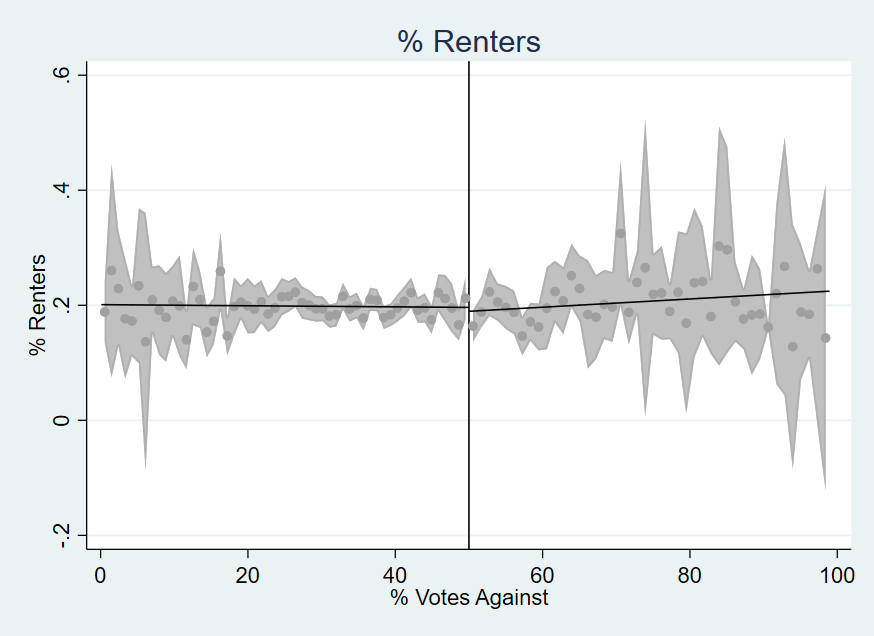
\includegraphics[width=\textwidth,keepaspectratio]{images/cov_smoothness_pctrent.png}
        \caption*{Pct Rent}
        \label{fig:pctrent_sm}
    \end{minipage}
    \hfill
    \begin{minipage}[b]{0.40\textwidth}
        \centering
        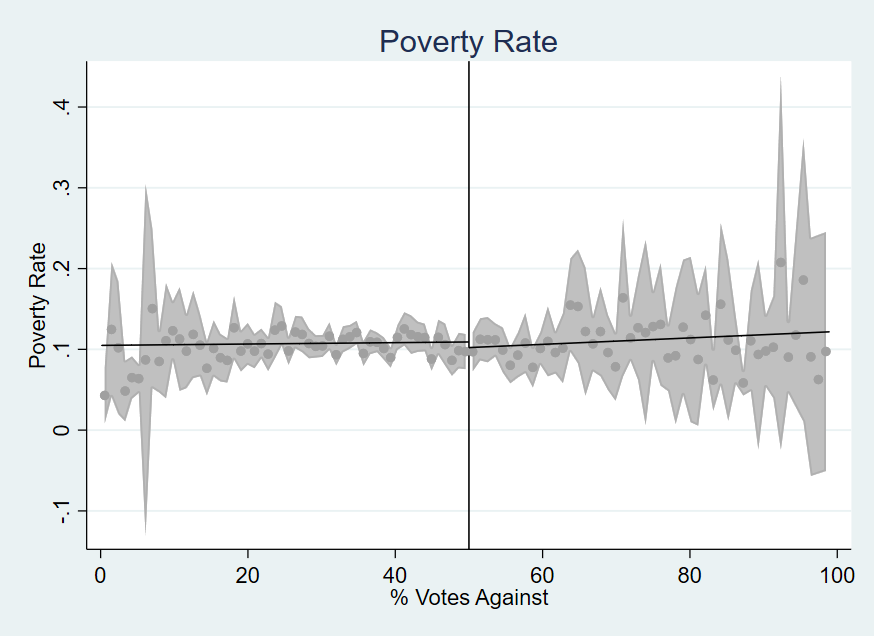
\includegraphics[width=\textwidth,keepaspectratio]{images/cov_smoothness_poverty.png}
        \caption*{Poverty Rate}
        \label{fig:poverty_sm}
    \end{minipage}
    
    % \vspace{1em}
    
    \begin{minipage}[b]{0.40\textwidth}
        \centering
        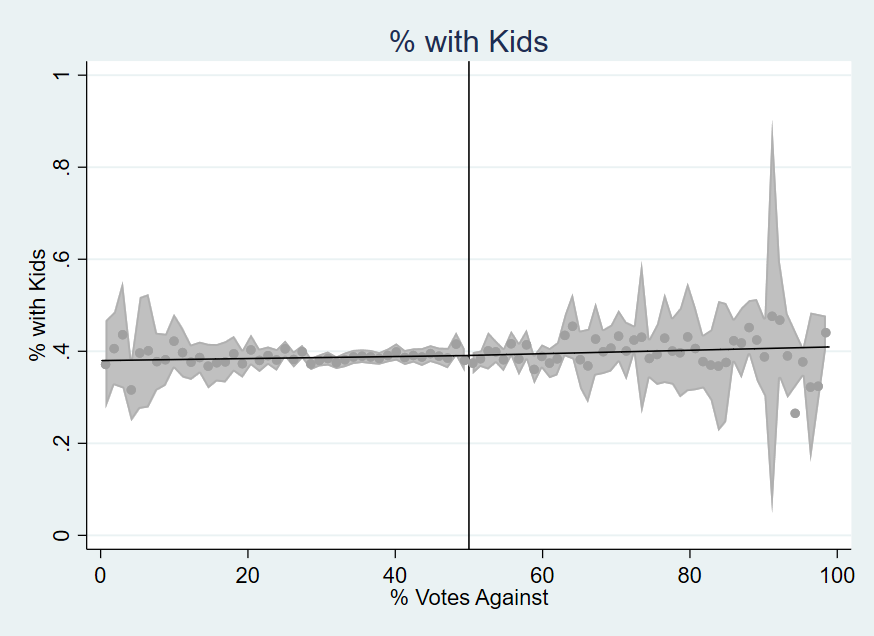
\includegraphics[width=\textwidth,keepaspectratio]{images/cov_smoothness_pctwithkids.png}
        \caption*{Pct With Kids}
        \label{fig:pct_with_kids_sm}
    \end{minipage}
    \hfill
    \begin{minipage}[b]{0.40\textwidth}
        \centering
        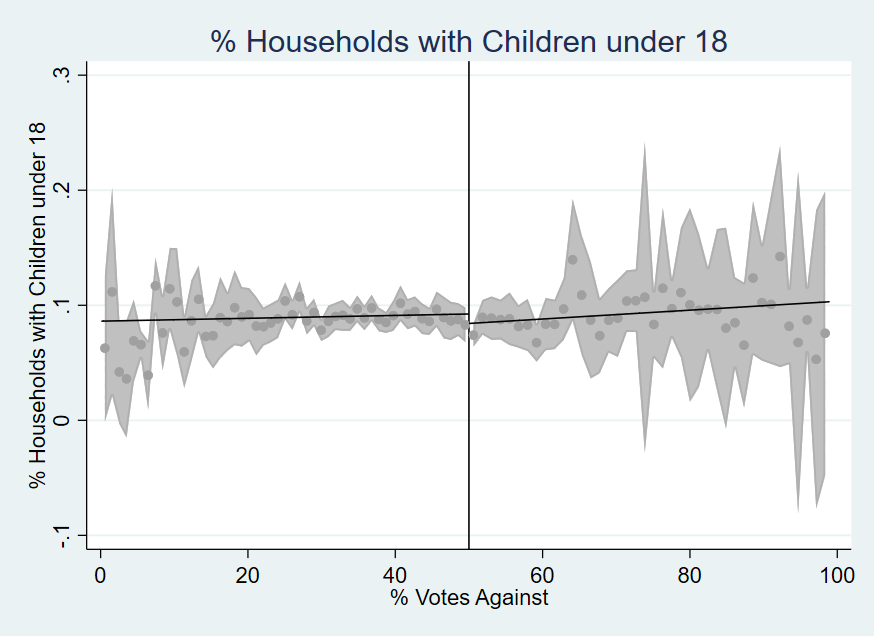
\includegraphics[width=\textwidth,keepaspectratio]{images/cov_smoothness_pctsinparhhld.png}
        \caption*{Pct Single Parent Hhld}
        \label{fig:pctsinparhhld_sm}
    \end{minipage}
    
    % \vspace{1em}
    
    \begin{minipage}[b]{0.40\textwidth}
        \centering
        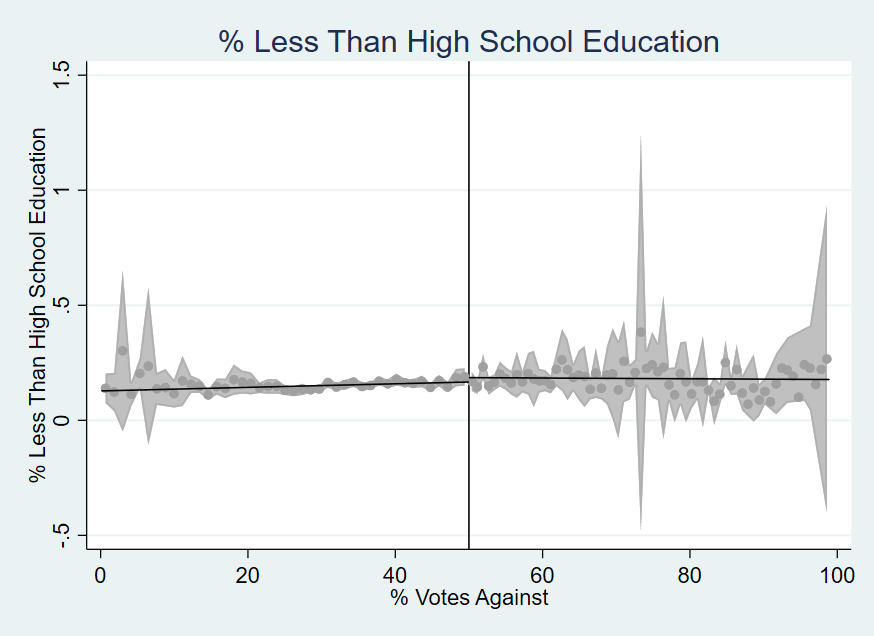
\includegraphics[width=\textwidth,keepaspectratio]{images/cov_smoothness_pctlesshs.png}
        \caption*{Pct Less than HS}
        \label{fig:pctlesshs_sm}
    \end{minipage}
    \hfill
    \begin{minipage}[b]{0.40\textwidth}
        \centering
        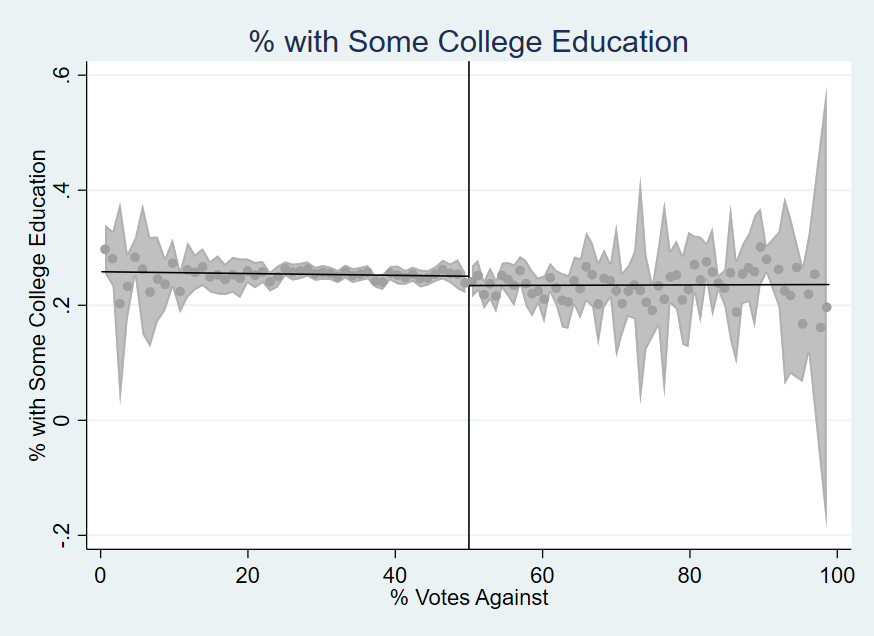
\includegraphics[width=\textwidth,keepaspectratio]{images/cov_smoothness_pctsomecoll.png}
        \caption*{Pct Some College}
        \label{fig:pctsomecoll_sm}
    \end{minipage}
    
    % \vspace{1em}
    
    \begin{minipage}[b]{0.40\textwidth}
        \centering
        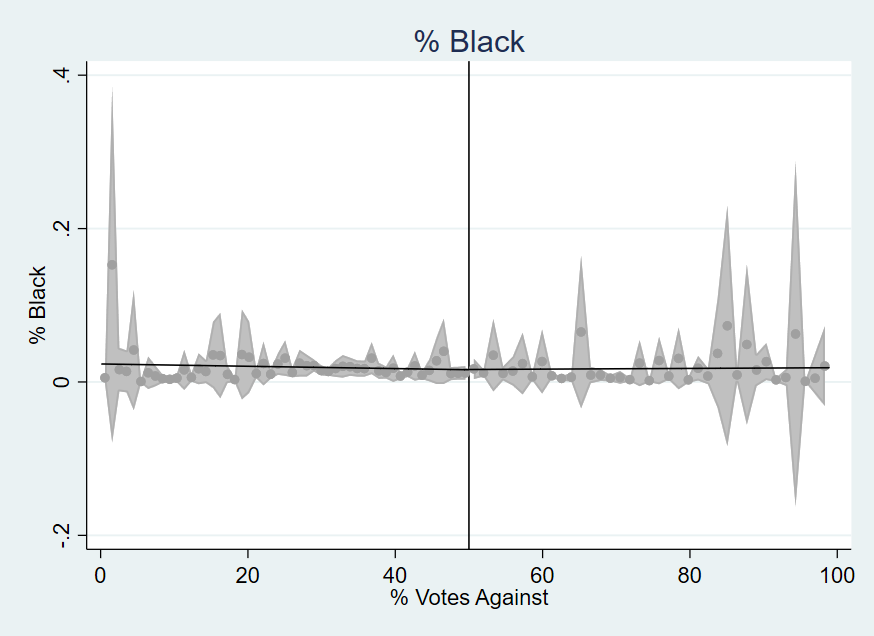
\includegraphics[width=\textwidth,keepaspectratio]{images/cov_smoothness_pctblack.png}
        \caption*{Pct Black}
        \label{fig:black_sm}
    \end{minipage}
    \hfill
    \begin{minipage}[b]{0.40\textwidth}
        \centering
        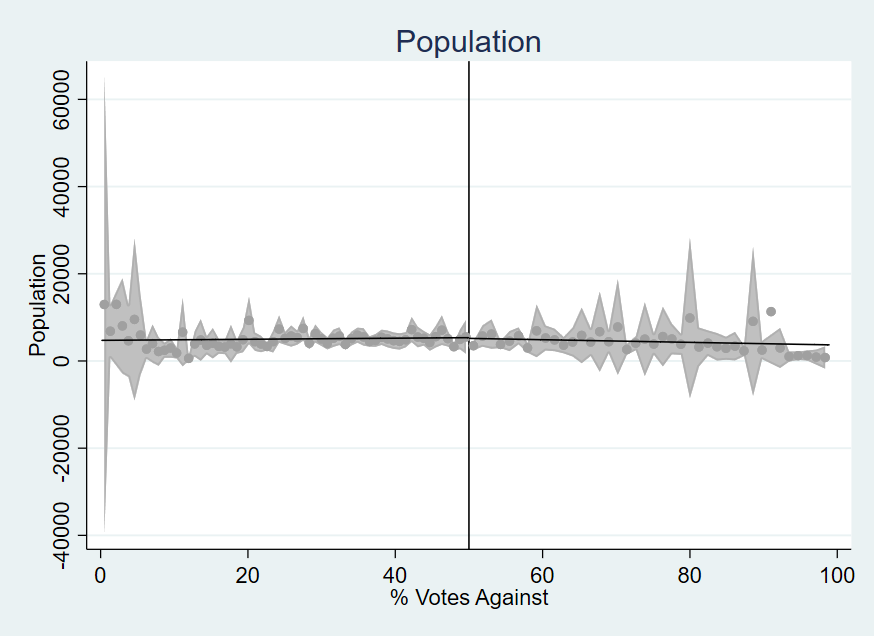
\includegraphics[width=\textwidth,keepaspectratio]{images/cov_smoothness_pop.png}
        \caption*{Population}
        \label{fig:pop_sm}
    \end{minipage}
    
    \caption{Covariate Discontinuity Plots - Part 1}
    \label{fig:rd_cov_smoothness_1}
\end{figure}

\begin{figure}[ht]
    \centering
    \begin{minipage}[b]{0.40\textwidth}
        \centering
        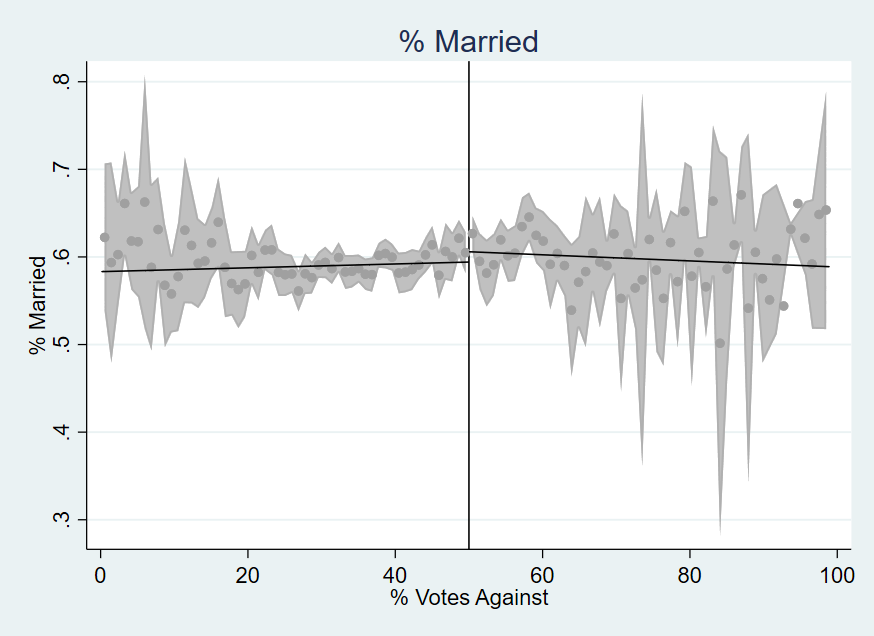
\includegraphics[width=\textwidth,keepaspectratio]{images/cov_smoothness_pctmarried.png}
        \caption*{Pct Married}
        \label{fig:pctmarried_sm}
    \end{minipage}
    \hfill
    \begin{minipage}[b]{0.40\textwidth}
        \centering
        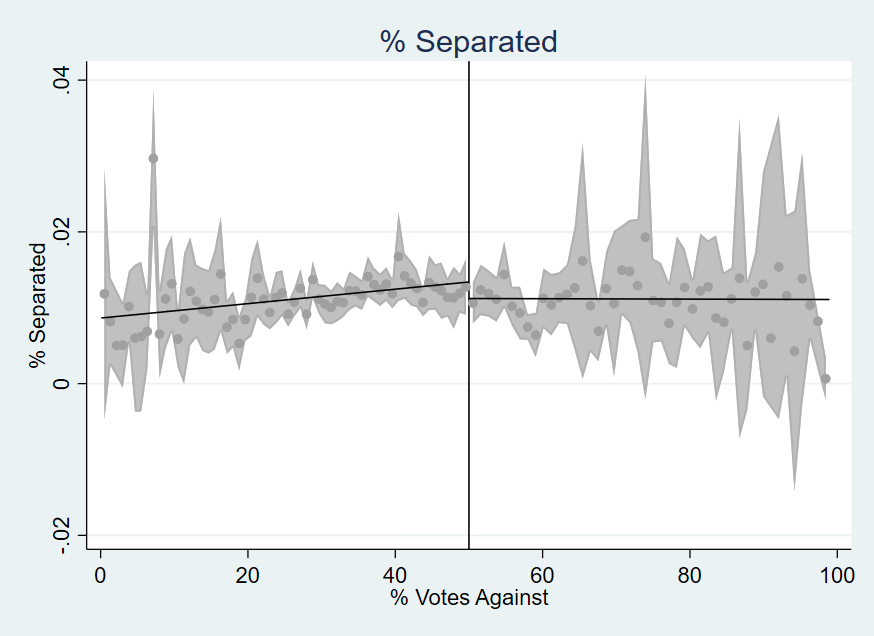
\includegraphics[width=\textwidth,keepaspectratio]{images/cov_smoothness_pctseparated.png}
        \caption*{Pct Separated}
        \label{fig:pctseparated_sm}
    \end{minipage}
    
    \vspace{1em}
    
    \begin{minipage}[b]{0.40\textwidth}
        \centering
        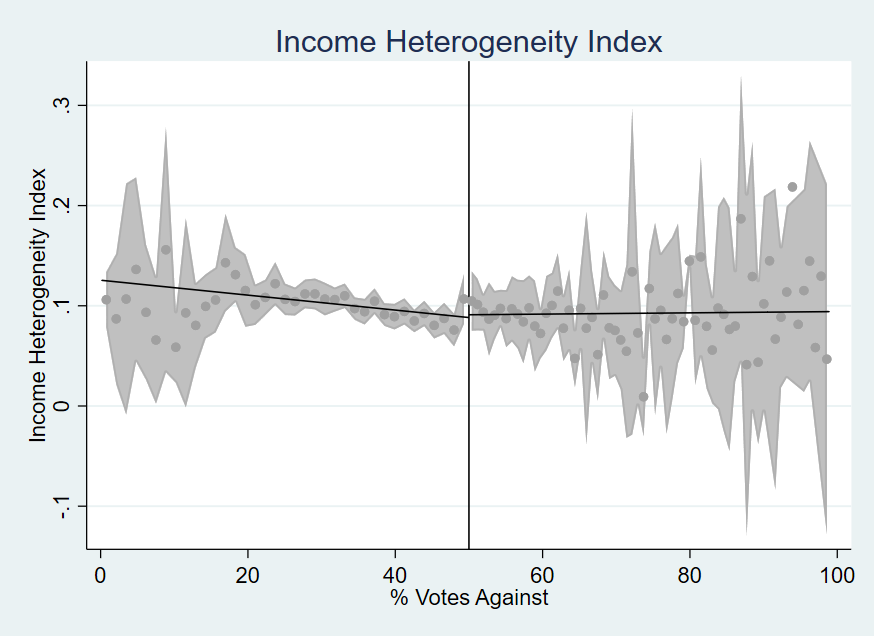
\includegraphics[width=\textwidth,keepaspectratio]{images/cov_smoothness_incherfindahl.png}
        \caption*{Income Herfindahl Index}
        \label{fig:incherfindahl_sm}
    \end{minipage}
    \hfill
    \begin{minipage}[b]{0.40\textwidth}
        \centering
        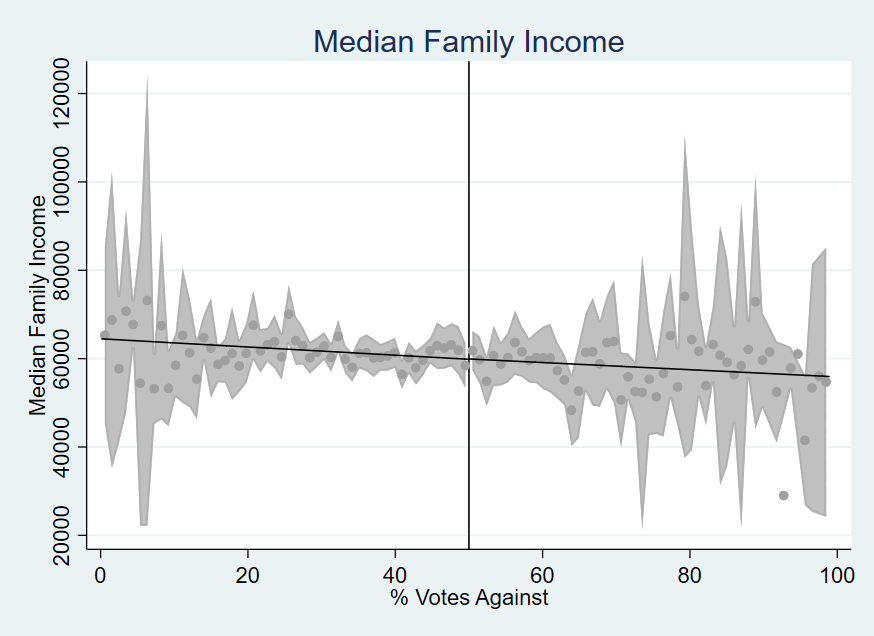
\includegraphics[width=\textwidth,keepaspectratio]{images/cov_smoothness_medfamy.png}
        \caption*{Median Family Income}
        \label{fig:medfamy_sm}
    \end{minipage}
    
    \vspace{1em}
    
    \begin{minipage}[b]{0.40\textwidth}
        \centering
        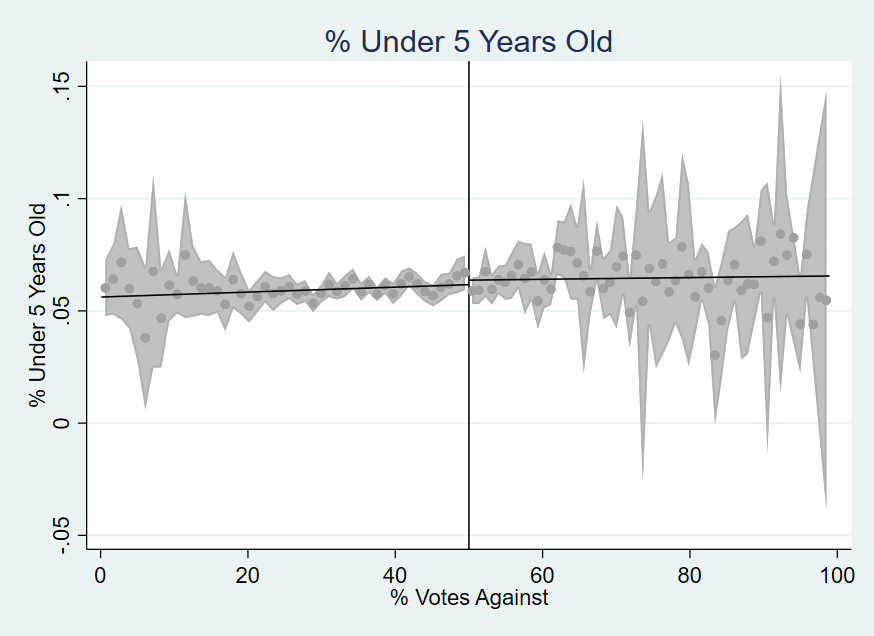
\includegraphics[width=\textwidth,keepaspectratio]{images/cov_smoothness_pctlt5.png}
        \caption*{Pct Less than 5}
        \label{fig:pctlt5_sm}
    \end{minipage}
    \hfill
    \begin{minipage}[b]{0.40\textwidth}
        \centering
        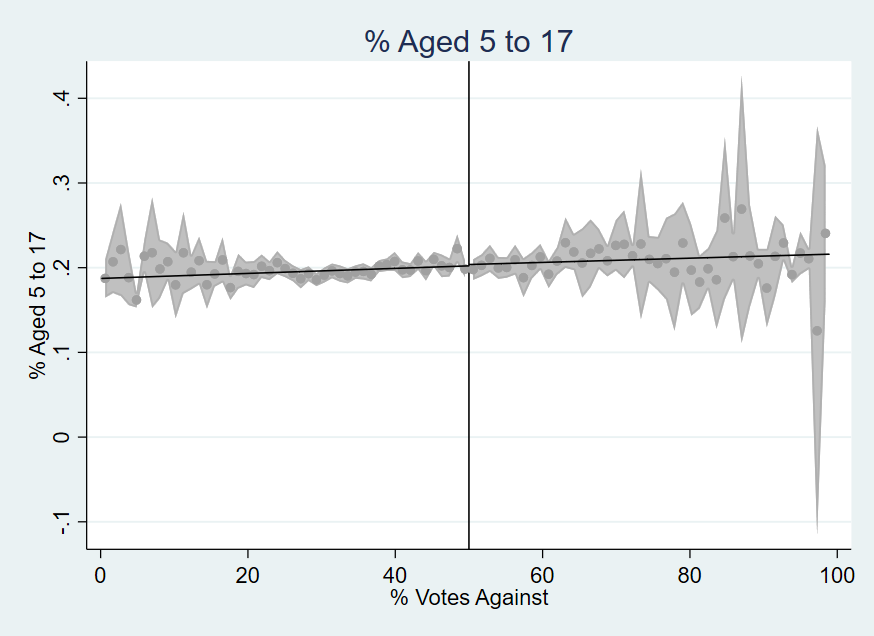
\includegraphics[width=\textwidth,keepaspectratio]{images/cov_smoothness_pct5to17.png}
        \caption*{Pct 5 to 17}
        \label{fig:pct5to17_sm}
    \end{minipage}
    
    \vspace{1em}
    
    \begin{minipage}[b]{0.40\textwidth}
        \centering
        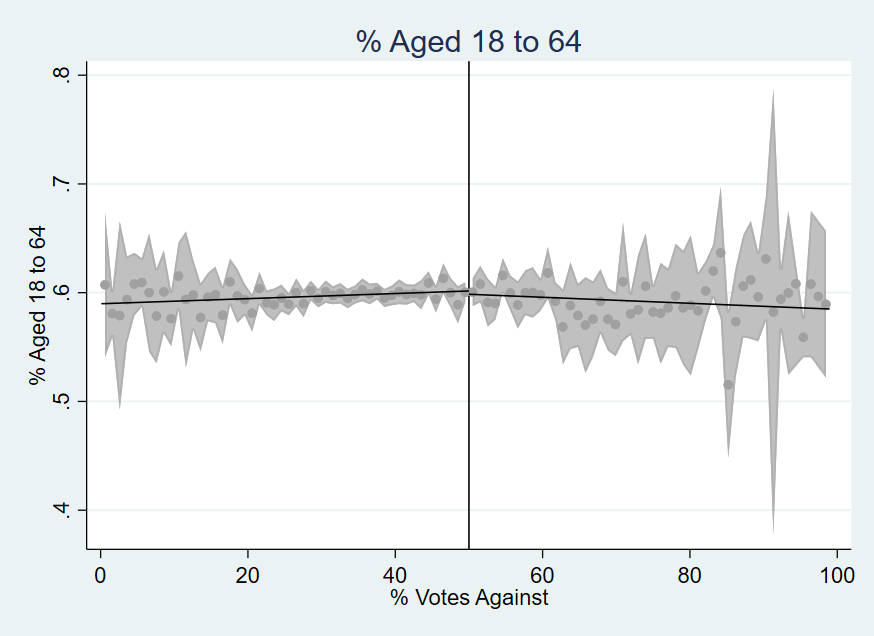
\includegraphics[width=\textwidth,keepaspectratio]{images/cov_smoothness_pct18to64.png}
        \caption*{Pct 18 to 64}
        \label{fig:pct18to64_sm}
    \end{minipage}
    \hfill
    \begin{minipage}[b]{0.40\textwidth}
        \centering
        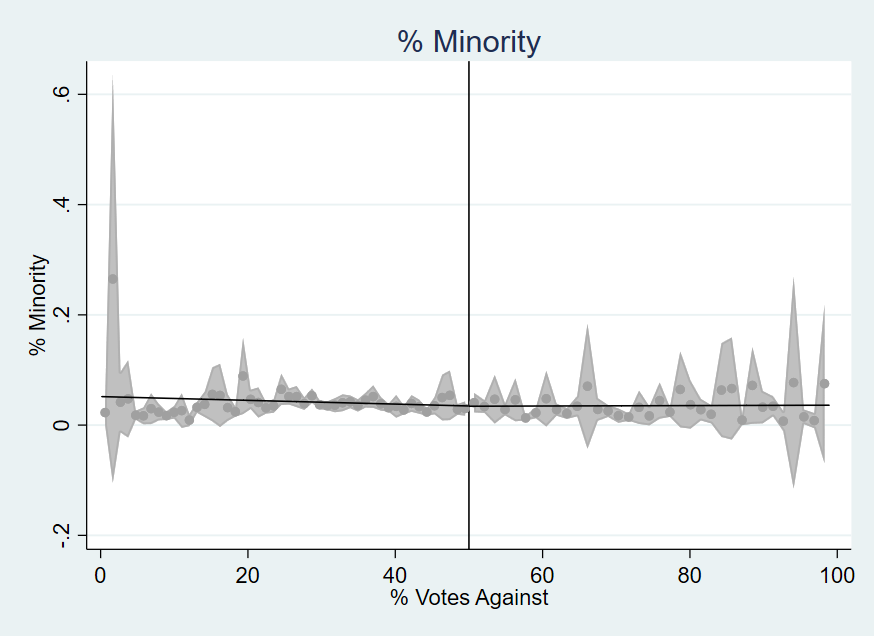
\includegraphics[width=\textwidth,keepaspectratio]{images/cov_smoothness_pctmin.png}
        \caption*{Pct Minority}
        \label{fig:pctmin_sm}
    \end{minipage}
    
    \caption{Covariate Discontinuity Plots - Part 2}
    \label{fig:rd_cov_smoothness_2}
\end{figure}


\clearpage


\section{Additional Information} \label{sec:appxc}

\subsection{A Case Study of Roads in Waynesville OH: Serial Cutter of Road Maintenance Tax Levies}

Coming very soon.

% \begin{figure}[ht]
%     \centering
%     \begin{minipage}[b]{0.48\textwidth}
%         \centering
%         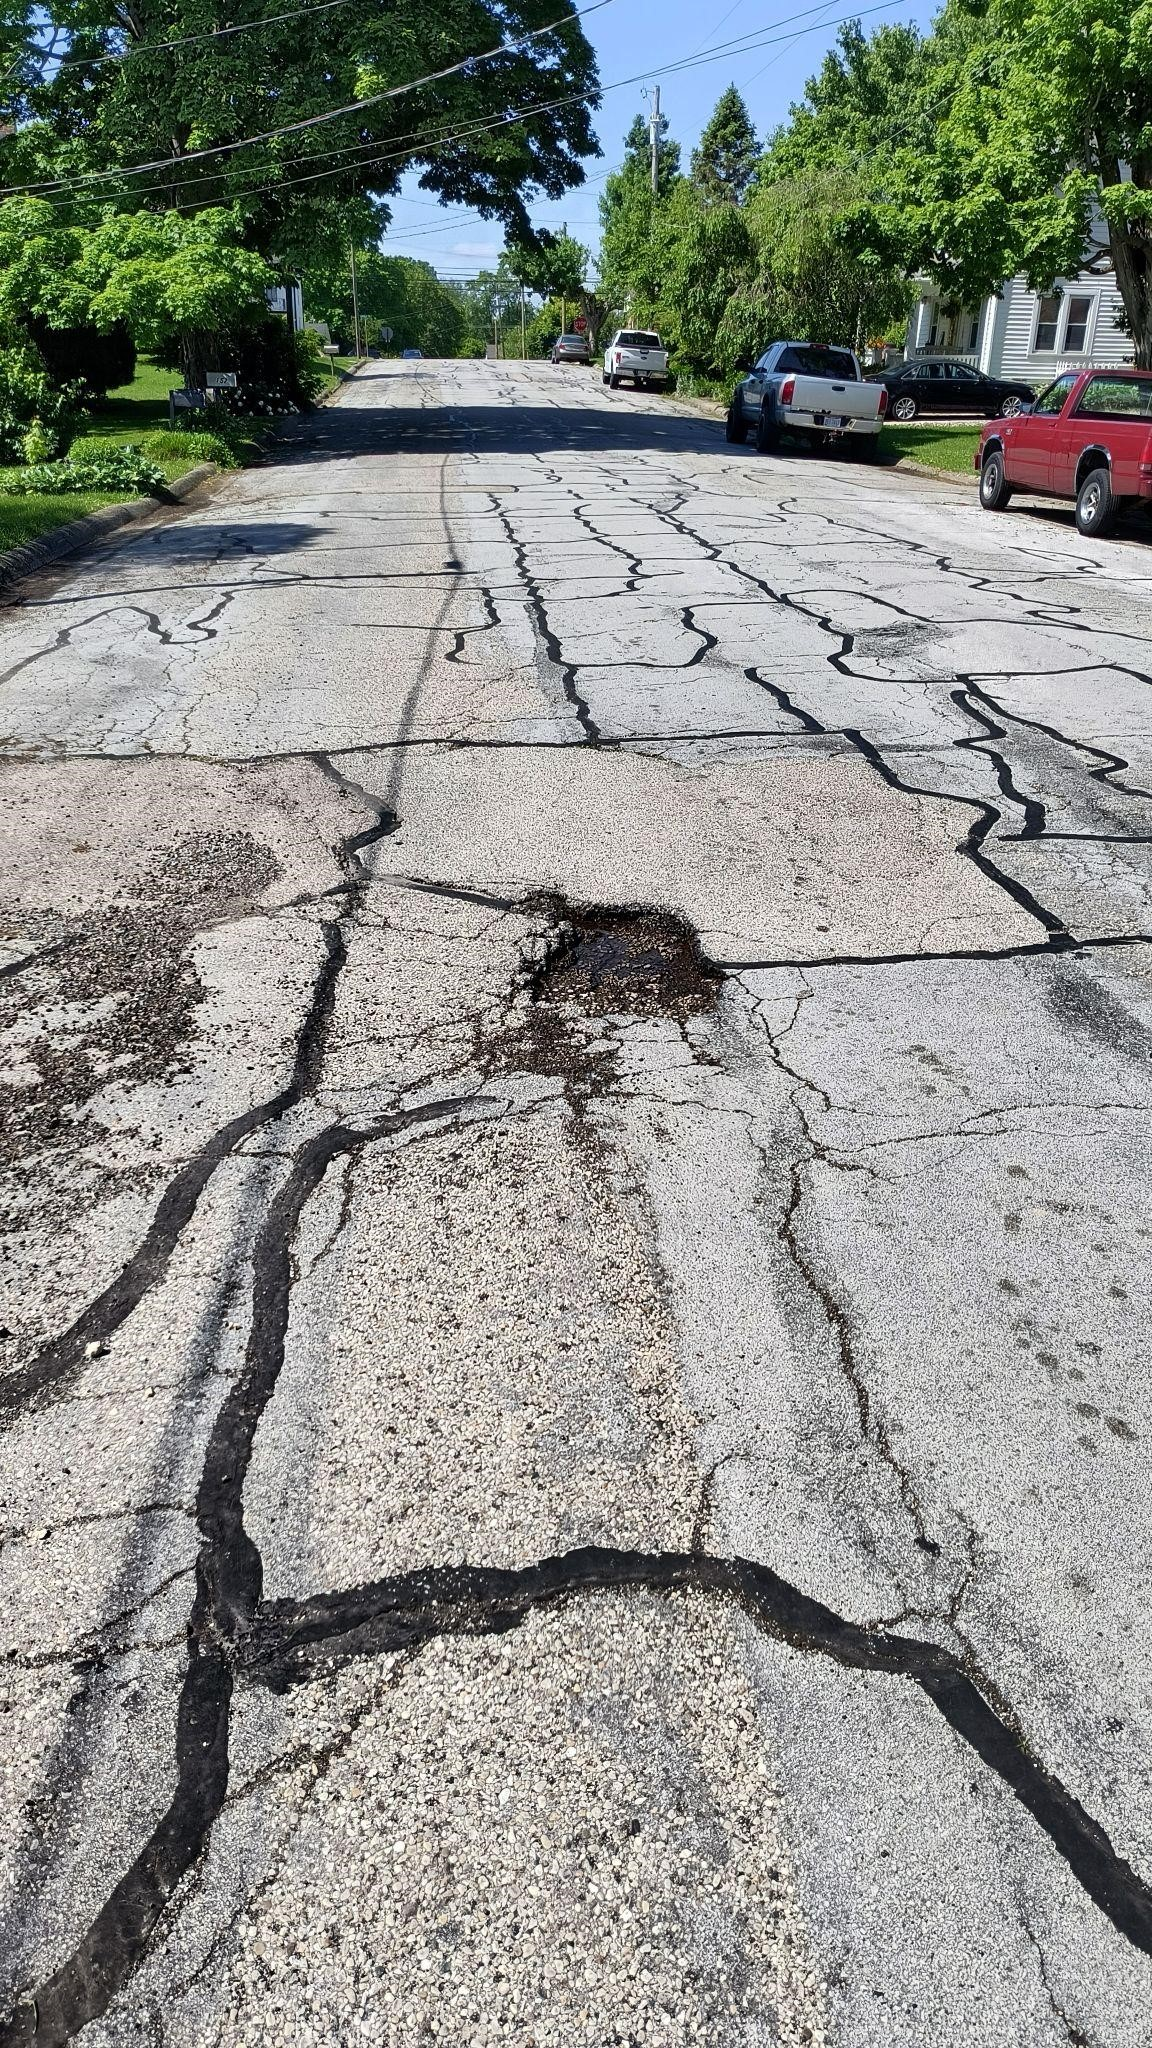
\includegraphics[width=0.75\textwidth,keepaspectratio]{images/waynesville_oh_1.png}
%         \caption*{Waynesville Road Image 1}
%         \label{fig:w_oh_1}
%     \end{minipage}
%     \hfill
%     \begin{minipage}[b]{0.48\textwidth}
%         \centering
%         \includegraphics[width=0.75\textwidth,keepaspectratio]{images/waynesville_oh_2.png}
%         \caption*{Waynesville Road Image 2}
%         \label{fig:w_oh_2}
%     \end{minipage}

%     \vspace{1em}

%     \begin{minipage}[b]{0.48\textwidth}
%         \centering
%         \includegraphics[width=0.75\textwidth,keepaspectratio]{images/waynesville_oh_3.png}
%         \caption*{Waynesville Road Image 3}
%         \label{fig:w_oh_3}
%     \end{minipage}

%     \caption{Roads in Waynesville: Case Study}
%     \label{fig:rd_waynesville}
% \end{figure}

